\documentclass[11pt,a4paper]{article}

% --- packages -------------------------------------------------------------
\usepackage[margin=1in]{geometry}
\usepackage{graphicx}
\usepackage{booktabs}
\usepackage{caption}
\usepackage{subcaption}
\usepackage{xcolor}
\usepackage{amsmath,amssymb}
\usepackage{siunitx}
\usepackage{microtype}
\usepackage{enumitem}
\usepackage{float}
\usepackage{tabularx}
\newcolumntype{Y}{>{\raggedright\arraybackslash}X}
\usepackage[hidelinks,colorlinks=true,linkcolor=NavyBlue,urlcolor=NavyBlue,citecolor=NavyBlue]{hyperref}
\usepackage[dvipsnames]{xcolor}

% Search path so we can use bare filenames across figure subdirectories
\graphicspath{%
  {./}%
  {../overview/}%
  {../heatmaps/}%
  {../direct/}%
  {../trait_aggregated/}%
  {../barplots/}%
  {../spatial_section/}%
  {../valve_enrichment_stats/}%
}

\captionsetup{font=small,labelfont=bf,labelsep=period}
\setlength{\parskip}{4pt}
\setlength{\parindent}{0pt}

% Define a custom callout box for "key takeaway"
\usepackage{tcolorbox}
\tcbset{colback=blue!4!white,colframe=blue!40!black,boxrule=0.4pt,
        arc=2pt,left=6pt,right=6pt,top=4pt,bottom=4pt}

% --- title ----------------------------------------------------------------
\title{\vspace{-1.5em}\textbf{A spatial atlas of cardiac-disease gene expression in the
PCW12 human fetal heart}\\[2pt]\large
End-to-end pipeline: cross-modal mapping, 3D spatial imputation,
cell-type enrichment, and trait--trait convergence}
\author{PCW12 Analysis Pipeline\thanks{Pipeline:
\texttt{PCW12\_analysis/scripts/01--12}.
Inputs: \texttt{all\_healthy\_RoundedPCW11-13.h5ad} (95{,}684 cells $\times$ 31{,}019 genes),
\texttt{full\_heart\_final\_aug2025\_update\_downsampled\_100k.h5ad} (100{,}000 cells $\times$ 238 genes),
\texttt{heart\_disease\_genes.tsv} (247 unique genes / 10 traits).}}
\date{\today}

% --- document -------------------------------------------------------------
\begin{document}
\maketitle

\begin{abstract}
\noindent We map a curated panel of 247 cardiac-disease genes onto a
3D MERFISH atlas of the post-conception week 12 (PCW12) human fetal heart
by combining a 95{,}684-cell scRNA-seq atlas (PCW 11--13) with a
100{,}000-cell MERFISH downsample. Of the 247 disease genes, 20 are
present on the 238-gene MERFISH panel (\emph{direct}); 221 are imputed by
optimal-transport mapping (MOSCOT, KL-balanced, $\alpha=0$,
$\tau_a=1$, $\tau_b=0.9$) over 229 cell-cycle-filtered shared genes;
6 are absent from both modalities. We then build (i) trait-aggregated 3D
expression maps for all 10 cardiac traits, (ii) per-gene peak-cell-type
assignments across the 34 PCW12 cell types, (iii) an anatomical valve
section (z-slice 16, 18.8\% valve cells, $\log_2$ enrichment $+2.52$),
(iv) a non-parametric Mann--Whitney U test of valve-cell trait
enrichment with a 2{,}000-permutation size-matched null and BH-FDR
control, and (v) a trait-by-celltype landscape with Yanai's $\tau$ and
Pearson/Jaccard trait--trait similarity. Three orthogonal expression
modules emerge --- working myocardium, AV/OFT cushion mesenchyme, and
aortic / general mesenchyme. HCM and DCM are nearly indistinguishable as
cell-type-resolved signatures ($r=0.998$) despite only 21\% gene
overlap. The TAA panel converges on the same cushion-mesenchymal cells
as the Valve\_defects panel ($r=0.85$) through only 3 shared genes ---
\emph{functional convergence via independent gene sets}. Six of ten
traits are statistically enriched in valve cells ($q_{\text{perm}}<0.05$);
HCM and DCM are correctly silent there, validating the test pipeline.
\end{abstract}

% =========================================================================
\section{Introduction}
\label{sec:intro}

A long-standing question in cardiac developmental genetics is whether
genes implicated in distinct cardiovascular phenotypes
(cardiomyopathies, septal defects, valve defects, conotruncal anomalies,
aortopathies) act through shared or distinct cellular programs during
heart formation. Bulk-tissue expression collapses this question;
high-resolution single-cell and 3D-spatial atlases of the developing
human heart now make it tractable.

This report walks through the full pipeline used to answer three
inter-locked questions on a curated 247-gene panel covering 10 cardiac
traits:
\begin{enumerate}[leftmargin=*,itemsep=0pt]
    \item \emph{Where} are disease genes expressed in the 3D fetal heart at PCW12?
    \item Which cell types are enriched for each disease gene set, and
          which valve subpopulations drive the strongest signals?
    \item When two traits converge on similar cell types, do they do so
          via shared genes or via independent genes that converge on the
          same developmental program?
\end{enumerate}

The answers depend on a chain of methods --- gene partitioning into
panel-direct vs.\ off-panel, optimal-transport mapping, anatomical
section selection, and three statistical summaries. We describe each in
turn (\S\ref{sec:methods}) and present results as eight self-contained
sections (\S\ref{sec:results}).

% =========================================================================
\section{Data and Methods}
\label{sec:methods}

\subsection{Input data}

\begin{table}[H]
    \centering\small
    \begin{tabularx}{\linewidth}{@{}l Y r r@{}}
        \toprule
        \textbf{Modality} & \textbf{File} & \textbf{Cells} & \textbf{Genes} \\
        \midrule
        scRNA-seq (PCW 11--13) & \texttt{all\_healthy\_RoundedPCW11-13.h5ad} & 95{,}684 & 31{,}019 \\
        MERFISH 3D (downsampled) & {\scriptsize\texttt{full\_heart\_final\_aug2025\_update\_\allowbreak downsampled\_100k.h5ad}} & 100{,}000 & 238 \\
        Disease panel & \texttt{heart\_disease\_genes.tsv} & --- & 247 unique \\
        \bottomrule
    \end{tabularx}
    \caption{Input modalities. The MERFISH dataset carries 3D
    coordinates in \texttt{obsm['X\_spateo\_update']} and curated
    \texttt{celltype} labels (34 fine classes); the scRNA-seq atlas
    carries the same fine-resolution annotation (after MOSCOT label
    transfer the two coincide on cell-type vocabulary). The disease
    panel covers ten traits: HCM, DCM, AVSD, OFT, ASD, VSD,
    Single-ventricle, Valve\_defects, TAA, and PCGC de-novo variants.
    Each gene may belong to multiple traits.}
\end{table}

\subsection{Gene partitioning}
\label{sec:methods:partition}
We partition the 247 disease genes by their availability across
modalities (\texttt{01\_partition\_genes.py}):
\begin{itemize}[leftmargin=*,itemsep=1pt]
    \item \textbf{Direct} (20 genes): in the MERFISH panel; visualised
          and analysed from the raw spatial counts.
    \item \textbf{Imputed} (221 genes): in scRNA-seq only; spatially
          imputed by MOSCOT optimal-transport mapping
          (\S\ref{sec:methods:moscot}).
    \item \textbf{Missing} (6 genes): \texttt{FOXE3}, \texttt{FOXH1},
          \texttt{GDF1}, \texttt{GET3}, \texttt{TAFAZZIN}, \texttt{ZIC3}
          --- absent from both. Excluded from all spatial analyses.
\end{itemize}

\subsection{MOSCOT optimal-transport mapping (scRNA $\to$ MERFISH)}
\label{sec:methods:moscot}

We use the scverse MOSCOT \texttt{MappingProblem} framework
(\texttt{03\_moscot\_imputation.py}) to learn a transport plan
$\pi \in \mathbb{R}_{\geq 0}^{n_{\text{sc}} \times n_{\text{sp}}}$ from
single cells to spatial cells. After log-normalisation of scRNA-seq
($\mathrm{normalize\_total}(10^4) \to \log\!1\!p$), we restrict to the
intersection of scRNA and MERFISH gene sets (237 shared) and remove
93 cell-cycle genes (S- and G2M-phase markers from
\texttt{omics/single\_cell\_basic\_qc}), leaving \textbf{229 mapping
genes}. The MERFISH dataset is split into \textbf{5 batches of 20{,}000
cells} (the smallest yields a tractable transport problem on CPU).
For each batch we solve
\[
\min_{\pi} \;
\underbrace{\langle \pi,\, C \rangle}_{\text{transport cost}}
+ \tau_a \, \mathrm{KL}\!\left(\pi \mathbf{1} \,\Vert\, a\right)
+ \tau_b \, \mathrm{KL}\!\left(\pi^{\!\top} \mathbf{1} \,\Vert\, b\right)
\]
with $C = \lVert U_{\text{sc}} - U_{\text{sp}}\rVert_2^2$ in a shared
local-PCA space (\texttt{xy\_callback="local-pca"}), $\alpha = 0$
(quadratic / GW term off; pure linear OT on shared genes),
$\tau_a = 1$ (balanced row marginals on scRNA-seq), and
$\tau_b = 0.9$ (slightly unbalanced column marginals on MERFISH, allowing
a small fraction of spatial cells to be ``unmatched''). Mean wall-clock
time is $\sim$130\,s per batch on CPU (no JAX Metal/CUDA backend on this
machine).

After solving, we scale the transport matrix by $\pi \leftarrow n_{\text{sc}}\,\pi$
so that columns sum to approximately one and impute disease-gene
expression (\S\ref{sec:methods:imputation}). Cell-type labels are
transferred by
\[
\hat{c}(j) \;=\; \arg\max_{k} \;\sum_{i \in \mathcal{C}_k} \pi_{ij}
\;=\; \arg\max_{k} \;[\pi^{\!\top} \mathbf{1}_{\text{onehot}}]_{j,k},
\]
i.e.\ the most-mass-voting source-celltype.

\subsection{Imputation of disease genes}
\label{sec:methods:imputation}
For the 221 off-panel disease genes, we set
\[
X_{\text{imp}} \;=\; \pi^{\!\top}\, X_{\text{sc}}\!\in\! \mathbb{R}^{n_{\text{sp}} \times 221},
\]
where $X_{\text{sc}}$ is the log-normalised scRNA-seq submatrix on those
221 genes. Per-batch outputs are concatenated into a single
\texttt{adata\_imputed\_disease\_genes.h5ad} (100{,}000 cells, 221 genes,
274 MB). MOSCOT mapping confidence (per-spatial-cell sum of top-1\%
transport mass) has mean 0.487, median 0.449, IQR 0.351--0.594 ---
moderate, as expected for unbalanced OT on a 229-gene cost.

\subsection{Trait scoring and per-celltype mean expression}
\label{sec:methods:trait_score}
The per-cell trait score is the mean log-normalised expression over the
trait's gene panel:
\[
s_{i,t} \;=\; \frac{1}{|\mathcal{G}_t|} \sum_{g \in \mathcal{G}_t} \mathrm{log1p}(\hat{x}_{i,g}).
\]
Per-celltype mean expression is
$\bar{X}_{g,c} = \frac{1}{|\mathcal{C}_c|} \sum_{i \in \mathcal{C}_c} \mathrm{log1p}(\hat{x}_{i,g})$,
yielding a $221 \times 34$ matrix. Trait-by-celltype enrichment is
$S_{t,c} = \frac{1}{|\mathcal{G}_t|} \sum_{g \in \mathcal{G}_t} z(\bar{X}_{g,c})$
with $z(\cdot)$ the across-celltype standardisation.

\subsection{Peak-cell-type assignment}
\label{sec:methods:peak}
For each of the 241 detectable disease genes (20 direct + 221 imputed)
we record
$\hat{c}_g = \arg\max_{c} \bar{X}_{g,c}$,
its peak cell type. Counting genes by their peak yields the per-cell-type
gene-count distribution (\S\ref{sec:res:peak},
\texttt{09\_disease\_genes\_peak\_celltype\_barplot.py}).

\subsection{Anatomical valve section}
\label{sec:methods:section}
The 3D MERFISH dataset contains 53 z-slices indexed by
\texttt{obs['section']}. We compute valve enrichment per section as
$\mathrm{frac\_valve} = (n_{\text{VIC}} + n_{\text{VEC}} + n_{\text{ncCM-AVC-like}})/n_{\text{section}}$
and pick \textbf{section 16} as the canonical valve plane: 440/2{,}337
valve cells (18.8\%), $\log_2$ enrichment $+2.52$ over the population
fraction (3.3\%). On this 2D plane we render trait scores as scatter
overlays (\texttt{10\_section16\_valve\_spatial.py}).

\subsection{Yanai's $\tau$, Pearson, Jaccard, hierarchical clustering}
\label{sec:methods:tau}
Per-gene specificity uses Yanai's index
\[
\tau_g = \frac{\sum_{c=1}^{K}(1 - \tilde{X}_{g,c})}{K-1},
\quad
\tilde{X}_{g,c} = \frac{\bar{X}_{g,c}}{\max_{c'}\bar{X}_{g,c'}},
\]
with $K=34$. Per trait pair $(t_1, t_2)$ we compute Pearson
correlation $r$ on $S_{t,\cdot}$ profiles and Jaccard overlap
$J = |\mathcal{G}_{t_1} \cap \mathcal{G}_{t_2}|/|\mathcal{G}_{t_1}\cup\mathcal{G}_{t_2}|$
on gene sets. Gene-by-celltype clustering uses Ward linkage on
Euclidean distance over $z$-scored rows.

\subsection{Valve enrichment statistics}
\label{sec:methods:stats}
Mann--Whitney U one-sided test (``score in valve $>$ score in non-valve''),
effect size reported as AUC. The headline statistic is a
\textbf{permutation $z$-score and BH-FDR-corrected $q$-value}: 2{,}000
random size-matched gene panels are drawn (without replacement) from
the 221-gene universe; each yields a null AUC, from which we compute
$z_{\text{perm}}$ and a two-sided $p$, then BH across the 10 traits to
$q_{\text{perm}}$. Robustness comparator: valve cells vs.\ other
mesenchymal cells (Compact / Trabecular / aFibro / adFibro / EPDC /
Proliferating vFibro), removing the trivial ``valve is not myocardium''
contrast (\S\ref{sec:res:stats},
\texttt{11\_valve\_enrichment\_stats.py}).

\subsection{Reproducibility}
The full pipeline is twelve numbered scripts under
\texttt{PCW12\_analysis/scripts/}; outputs land in
\texttt{PCW12\_analysis/figures/} (subdirectories per phase) and
\texttt{PCW12\_analysis/data/}. See the Data and Code Availability
section for a one-shot reproduction recipe.

% =========================================================================
\section{Results}
\label{sec:results}

\subsection{Cross-modal data overview}
\label{sec:res:overview}

\begin{figure}[H]
    \centering
    \begin{subfigure}[t]{0.34\linewidth}
        
\includegraphics[width=\linewidth]{scrna_celltype.png}
        \caption{scRNA-seq composition (11 broad classes).}
    \end{subfigure}\hfill
    \begin{subfigure}[t]{0.32\linewidth}
        
\includegraphics[width=\linewidth]{merfish_celltype.png}
        \caption{MERFISH composition (34 fine classes).}
    \end{subfigure}\hfill
    \begin{subfigure}[t]{0.30\linewidth}
        
\includegraphics[width=\linewidth]{crossmod_overlap.png}
        \caption{Cross-modality cell-type composition.}
    \end{subfigure}
    \caption{\textbf{Cross-modal data overview.} Cell-type counts
    across the two modalities. The scRNA-seq atlas (95{,}684 cells)
    annotates 11 broad classes (a); the MERFISH 3D downsample
    (100{,}000 cells) annotates 34 fine classes (b); cross-modality
    overlap (c) compares broad-class proportions after MOSCOT
    label-mapping of MERFISH onto the scRNA-seq vocabulary. Broadly
    comparable proportions across the major lineages support
    cross-modal transport (\S\ref{sec:res:mapping}). Spatial UMAPs
    (scRNA-seq) and 3D scatter (MERFISH) are in
    \texttt{figures/overview/}.}
    \label{fig:overview}
\end{figure}

\subsection{MOSCOT mapping recovers cell-type identity}
\label{sec:res:mapping}

\begin{figure}[H]
    \centering
    
\includegraphics[width=\linewidth]{mapping_coarseSC_x_spatialFine.png}
    \caption{\textbf{Coarse-source$\,\times\,$fine-target transport
    matrix.} Each column is a MERFISH spatial cell type; each row a
    coarse scRNA-seq lineage (VCM, ACM, FB, Endocardial, Endothelial,
    MuralCells, Epicardial, Conduction, Myeloid/Lymphoid, Neuronal/NC).
    Column-normalised mass: each spatial cell type sums to 1. Strong
    diagonal recovery is evident (vCM-LV/RV-Compact $\to$ VCM at
    0.78--0.98; aCM-LA/RA $\to$ ACM at 0.78--0.84; valve / fibro target
    types $\to$ FB at 0.85--0.99). The Conduction-cell signal is
    correctly concentrated on \texttt{vCM-LV/RV-Purkinje} (0.84) and
    \texttt{vCM-IVS-His} (0.45). MyeloidCells $\to$ \texttt{WBC} at 0.84.
    The matrix is sparse off-diagonal --- a non-trivial validation of
    the transport plan.}
    \label{fig:mapping}
\end{figure}

\textbf{Quality verdict.} Mean confidence 0.487, median 0.449
(IQR 0.351--0.594) is moderate, as expected for unbalanced OT mapping
on a 229-gene cost; cell-type-level patterns are recovered cleanly but
single-cell resolution should not be over-interpreted on imputed values.

\subsection{Direct 3D visualisation: sanity-check disease genes}
\label{sec:res:direct}

\begin{figure}[H]
    \centering
    \begin{subfigure}[t]{0.49\linewidth}
        
\includegraphics[width=\linewidth]{MYH11.png}
        \caption{\textbf{MYH11} (TAA) --- VSMC-restricted, focal in the aortic rim.}
    \end{subfigure}\hfill
    \begin{subfigure}[t]{0.49\linewidth}
        
\includegraphics[width=\linewidth]{NOTCH1.png}
        \caption{\textbf{NOTCH1} (Valve / OFT) --- endocardial + LEC.}
    \end{subfigure}\\[6pt]
    \begin{subfigure}[t]{0.49\linewidth}
        
\includegraphics[width=\linewidth]{JAG1.png}
        \caption{\textbf{JAG1} (OFT / Alagille) --- neuronal + adventitial fibroblast.}
    \end{subfigure}\hfill
    \begin{subfigure}[t]{0.49\linewidth}
        
\includegraphics[width=\linewidth]{TBX5.png}
        \caption{\textbf{TBX5} (CHD TF) --- broad ventricular trabecular CM and atrial.}
    \end{subfigure}
    \caption{\textbf{Direct 3D expression of four canonical disease
    genes} measured on the MERFISH panel
    (\texttt{02\_direct\_visualization.py}; PyVista off-screen scatter on
    \texttt{X\_spateo\_update}, $\mathrm{log1p}$ colour). All four
    localise as expected from prior literature, validating the spatial
    coordinate system and the cell-type assignment. Full set of 20
    direct-gene panels in \texttt{figures/direct/}.}
    \label{fig:direct}
\end{figure}

\subsection{Trait-aggregated 3D maps}
\label{sec:res:trait3d}

\begin{figure}[H]
    \centering
    
\includegraphics[width=\linewidth]{_summary_panel.png}
    \caption{\textbf{Trait-aggregated 3D expression maps}
    (\texttt{05b\_trait\_aggregation.py}). Each panel shows 100{,}000
    MERFISH cells coloured by the per-cell trait score
    (mean $\log\!1\!p$ over the trait's gene panel, then within-trait
    $z$-scored). Traits are arranged from largest panel (top-left,
    Atrial septal defect, $n=88$) to smallest (bottom, Familial thoracic
    aortic aneurysm, $n=9$). The myocardial cardiomyopathy panels (HCM,
    DCM) light up the central ventricular mass; the cushion-mesenchymal
    traits (Valve defects, AVSD, OFT, TAA) light up the valve / aortic
    rim. Animated (GIF) versions in \texttt{figures/trait\_aggregated/}.}
    \label{fig:trait3d}
\end{figure}

\subsection{Peak-cell-type assignment of disease genes}
\label{sec:res:peak}

\begin{figure}[H]
    \centering
    
\includegraphics[width=\linewidth]{disease_gene_peak_celltype_barplot.pdf}
    \caption{\textbf{Number of disease genes whose mean expression peaks
    in each cell type} (\texttt{09\_disease\_genes\_peak\_celltype\_barplot.py}).
    241 detectable disease genes; cell types ordered within their lineage,
    bars coloured by lineage. The peaks distribute broadly across all
    nine lineages, with the largest single bins in the working ventricular
    myocardium (\texttt{vCM-RV-Compact} $n=26$, \texttt{vCM-RV-Proliferating}
    $n=12$), the AV-canal myocardium (\texttt{ncCM-AVC-like} $n=16$), and
    the endothelial / fibroblast / immune compartments
    (\texttt{BEC} $n=15$, \texttt{adFibro} $n=15$, \texttt{WBC} $n=15$,
    \texttt{LEC} $n=14$, \texttt{aEndocardial} $n=14$).}
    \label{fig:peak}
\end{figure}

\begin{table}[H]
    \centering\small
    \begin{tabular}{@{}lll r@{\hspace{2.0em}}lll r@{}}
        \toprule
        \textbf{Cell type} & \textbf{Lineage} & & \textbf{$n$} &
        \textbf{Cell type} & \textbf{Lineage} & & \textbf{$n$} \\
        \midrule
        vCM-RV-Compact          & vCM         & & 26 & adFibro              & Fibroblast & & 15 \\
        ncCM-AVC-like           & ncCM        & & 16 & WBC                  & Immune     & & 15 \\
        BEC                     & Endothelial & & 15 & LEC                  & Endothelial & & 14 \\
        aEndocardial            & Endothelial & & 14 & vCM-RV-Proliferating & vCM        & & 12 \\
        Neuronal                & Neural      & & 11 & VEC                  & Endothelial & & 11 \\
        vCM-LV-Hybrid           & vCM         & & 11 & aCM-LA               & aCM        & & 11 \\
        \bottomrule
    \end{tabular}
    \caption{Top peak-cell-type bins (12/34 cell types shown; full
    counts in \texttt{disease\_gene\_peak\_celltype\_counts.tsv}). The
    distribution spans every major lineage --- a useful auditing
    summary that no single lineage monopolises the panel.}
    \label{tab:peak}
\end{table}

\subsection{Valve anatomical section}
\label{sec:res:section}

\begin{figure}[H]
    \centering
    \begin{subfigure}[t]{0.42\linewidth}
        
\includegraphics[width=\linewidth]{section16_valve_celltypes.pdf}
        \caption{Valve cell types on section 16.}
        \label{fig:section:cells}
    \end{subfigure}\hfill
    \begin{subfigure}[t]{0.56\linewidth}
        
\includegraphics[width=\linewidth]{section16_disease_trait_panels.pdf}
        \caption{Trait-score panels for all 10 traits.}
        \label{fig:section:traits}
    \end{subfigure}
    \caption{\textbf{Section 16 --- the most valve-enriched z-slice}
    (\texttt{10\_section16\_valve\_spatial.py}; 2{,}337 cells, 18.8\%
    valve, $\log_2$ enrichment $+2.52$).
    (\subref{fig:section:cells}) Three valve-associated cell types
    over a light-grey section background: VIC (magenta), VEC (green),
    ncCM-AVC-like (blue). The VIC/VEC ring delineates the AV-canal
    cushion; ncCM-AVC-like sits in the underlying myocardium.
    (\subref{fig:section:traits}) Per-cell trait scores
    (within-trait $z$). The cushion-mesenchymal traits (Valve defects,
    AVSD, OFT, TAA) co-localise with the VIC/VEC ring; the cardiomyopathy
    panels (HCM, DCM) instead light up the central myocardial mass ---
    a visual confirmation of the cell-type-resolved enrichment patterns
    in \S\ref{sec:res:landscape}.}
    \label{fig:section}
\end{figure}

\subsection{Valve enrichment statistics}
\label{sec:res:stats}

\begin{figure}[H]
    \centering
    \begin{subfigure}[t]{0.49\linewidth}
        
\includegraphics[width=\linewidth]{fig1_bar_auc.pdf}
        \caption{Per-trait AUC (valve vs.\ non-valve). 0.5 = no enrichment.}
    \end{subfigure}\hfill
    \begin{subfigure}[t]{0.49\linewidth}
        
\includegraphics[width=\linewidth]{fig2_volcano.pdf}
        \caption{Permutation $z$ vs.\ $\log_2$FC volcano.}
    \end{subfigure}
    \caption{\textbf{Mann--Whitney enrichment of disease-trait scores
    in valve cells} ($n=3{,}278$ valve, $n=96{,}722$ non-valve;
    \texttt{11\_valve\_enrichment\_stats.py}). Six of ten traits are
    enriched at $q_{\text{perm}} < 0.05$ (Familial TAA, Valve defects,
    AVSD, OFT malformation, PCGC, Single-ventricle disease borderline);
    HCM and DCM are correctly depleted (the working-myocyte panels are
    \emph{absent} from valve cells), validating the test pipeline.
    Numbers and per-subtype break-down in Table~\ref{tab:stats}.}
    \label{fig:stats}
\end{figure}

\begin{table}[H]
    \centering\small
    \begin{tabularx}{\linewidth}{@{}l r r r r r Y@{}}
        \toprule
        \textbf{Trait} & \textbf{$k$} & \textbf{AUC} & \textbf{$\log_2$FC} & \textbf{$z_{\text{perm}}$} & \textbf{$q_{\text{perm}}$} & \textbf{Verdict} \\
        \midrule
        Familial TAA                & 9  & \textbf{0.775} & $+0.43$ & $+2.5$ & $3.0\!\times\!10^{-3}$ & enriched \\
        Valve defects               & 74 & \textbf{0.757} & $+0.22$ & $+7.6$ & $1.2\!\times\!10^{-3}$ & enriched \\
        AV septal defect            & 23 & \textbf{0.726} & $+0.21$ & $+2.5$ & $7.5\!\times\!10^{-3}$ & enriched \\
        OFT malformation            & 57 & \textbf{0.725} & $+0.18$ & $+4.7$ & $1.2\!\times\!10^{-3}$ & enriched \\
        PCGC de-novo                & 61 & 0.631 & $+0.09$ & $+4.1$ & $1.2\!\times\!10^{-3}$ & enriched \\
        Single ventricle            & 17 & 0.625 & $+0.13$ & $+1.7$ & $4.7\!\times\!10^{-2}$ & borderline \\
        Atrial septal defect        & 88 & 0.551 & $+0.03$ & $+6.3$ & $1.2\!\times\!10^{-3}$ & weak (small effect) \\
        Ventricular septal defect   & 34 & 0.475 & $-0.02$ & $+1.6$ & $7.1\!\times\!10^{-2}$ & n.s. \\
        Dilated cardiomyopathy      & 41 & 0.181 & $-1.43$ & $-12.7$ & $1.0$ & depleted (control) \\
        Hypertrophic cardiomyopathy & 27 & 0.177 & $-2.01$ & $-13.4$ & $1.0$ & depleted (control) \\
        \bottomrule
    \end{tabularx}
    \caption{Valve vs.\ non-valve enrichment by trait. AUC $=$
    P(score(random valve cell) $>$ score(random non-valve cell)).
    The bottom two rows are the working-myocyte panels and are
    correctly depleted in valve cells.}
    \label{tab:stats}
\end{table}

\textbf{Per-subtype drivers} (Mann--Whitney AUC vs.\ all non-valve, top
hit per valve subtype): VIC ($n=2{,}372$) drives the connective-tissue
signal --- Familial TAA AUC $0.826$, Valve defects $0.764$, OFT
malformation $0.753$. VEC ($n=720$) drives the endocardial-cushion
signal --- AVSD AUC $0.799$, Valve defects $0.781$.
ncCM-AVC-like ($n=186$) is a myocardial population at the AV junction
and drives septal-CHD signal --- Single-ventricle $0.651$, VSD $0.646$,
ASD $0.608$.

\begin{tcolorbox}
\textbf{TAA caveat.} The TAA panel scores high vs.\ all-non-valve
(AUC $0.775$) but \emph{lower than fibroblasts} when those are used as
the comparator (AUC $0.414$ vs.\ Compact / Trabecular / aFibro / adFibro
/ EPDC / Proliferating vFibro). TAA is therefore a generic mesenchymal
signature shared with fibroblasts, not valve-specific --- a useful
caveat for any naive valve-vs-rest test. This finding re-appears at
the celltype-profile level in \S\ref{sec:res:landscape}, where TAA and
Valve\_defects converge on the same cushion-mesenchymal program through
\emph{different} genes ($r=0.85$, only 3 shared genes).
\end{tcolorbox}

\subsection{Disease-gene landscape: trait-by-celltype, gene specificity, and trait--trait similarity}
\label{sec:res:landscape}

This section replays the four-figure landscape report on the same
imputed expression matrix used for the spatial maps and the valve test
above. We compute (i) trait-by-celltype $z$-scores, (ii) Yanai's $\tau$
per gene, and (iii) Pearson / Jaccard trait--trait similarity, all on
the $221 \times 34$ per-celltype mean matrix.

\subsubsection{Trait--celltype landscape: two reciprocal blocks}

\begin{figure}[H]
    \centering
    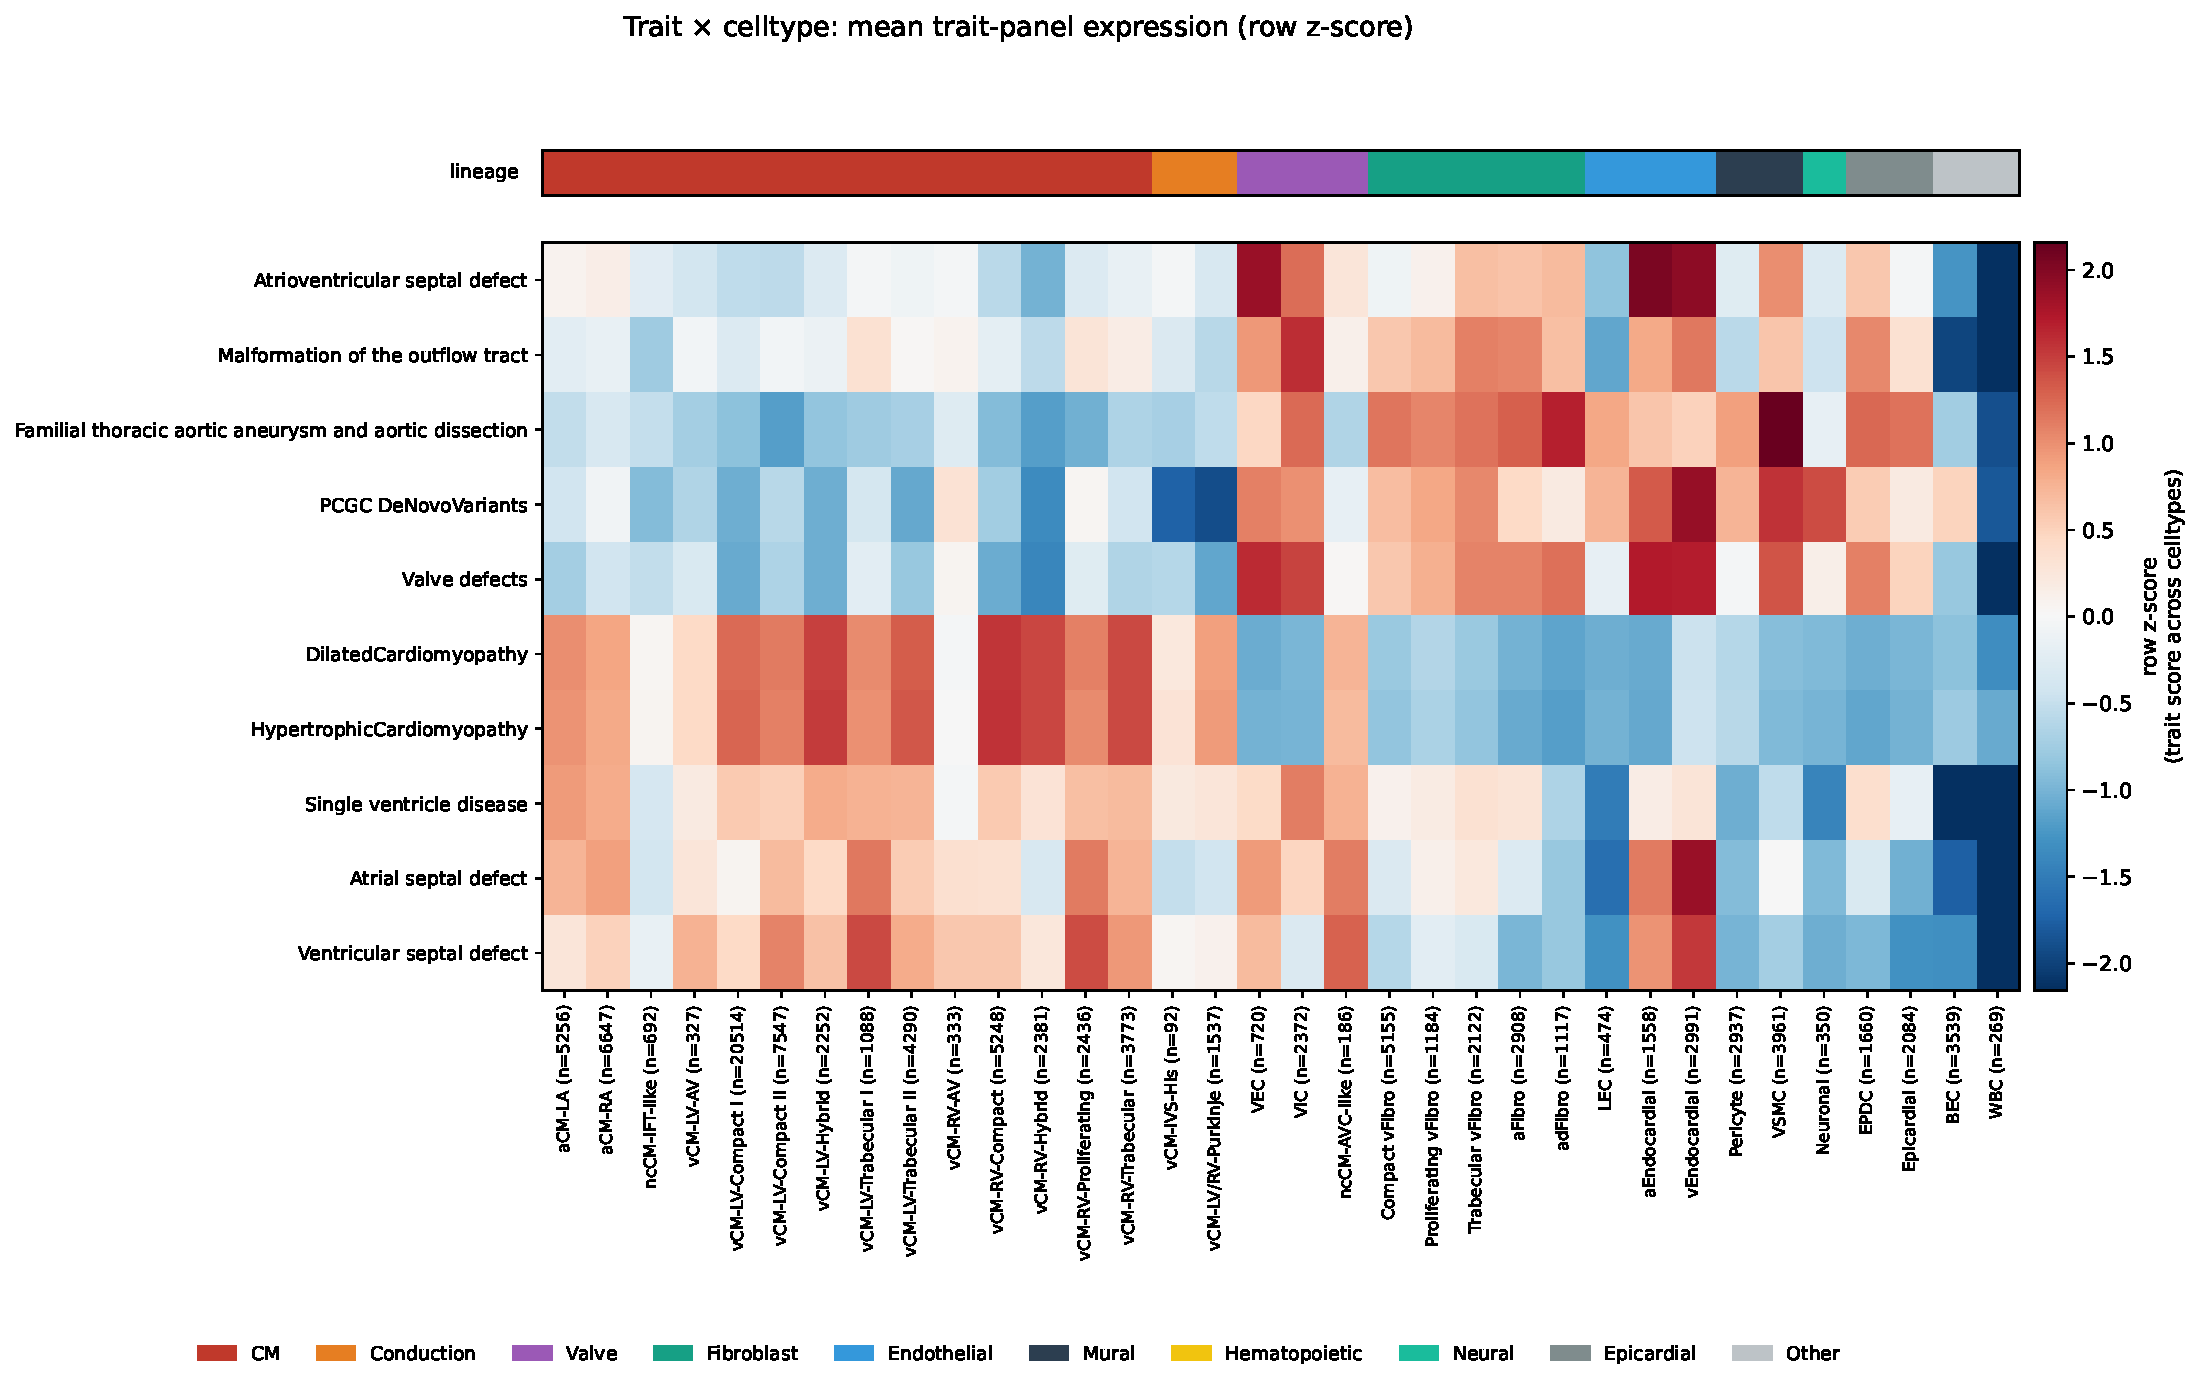
\includegraphics[width=0.95\linewidth]{figA_trait_by_celltype.pdf}
    \caption{\textbf{Trait-by-celltype enrichment.} Rows: 10 cardiac-disease
    traits. Columns: 34 PCW12 cell types ordered by developmental
    lineage (coloured strip above the heatmap). Two reciprocal blocks
    emerge: HCM/DCM peak in working ventricular cardiomyocytes, whereas
    Valve\_defects, AVSD, OFT, TAA, PCGC and ASD/VSD/Single-ventricle
    peak in valve endothelial / interstitial cells, endocardium, and
    mesenchymal fibroblasts / VSMC.}
    \label{fig:A}
\end{figure}

The trait-by-celltype heatmap (Fig.~\ref{fig:A}) shows two qualitatively
distinct enrichment patterns. Beyond the obvious myocardial vs.\ cushion
split, two negative-control observations are equally informative:
\textbf{WBC} and \textbf{BEC} are pan-blue across all 10 traits,
indicating that the panel carries essentially no hematopoietic or
capillary-endothelial signal at PCW12 and these cell types make natural
biological negative controls in any downstream gene-set test.

\subsubsection{Three unsupervised gene modules}

\begin{figure}[H]
    \centering
    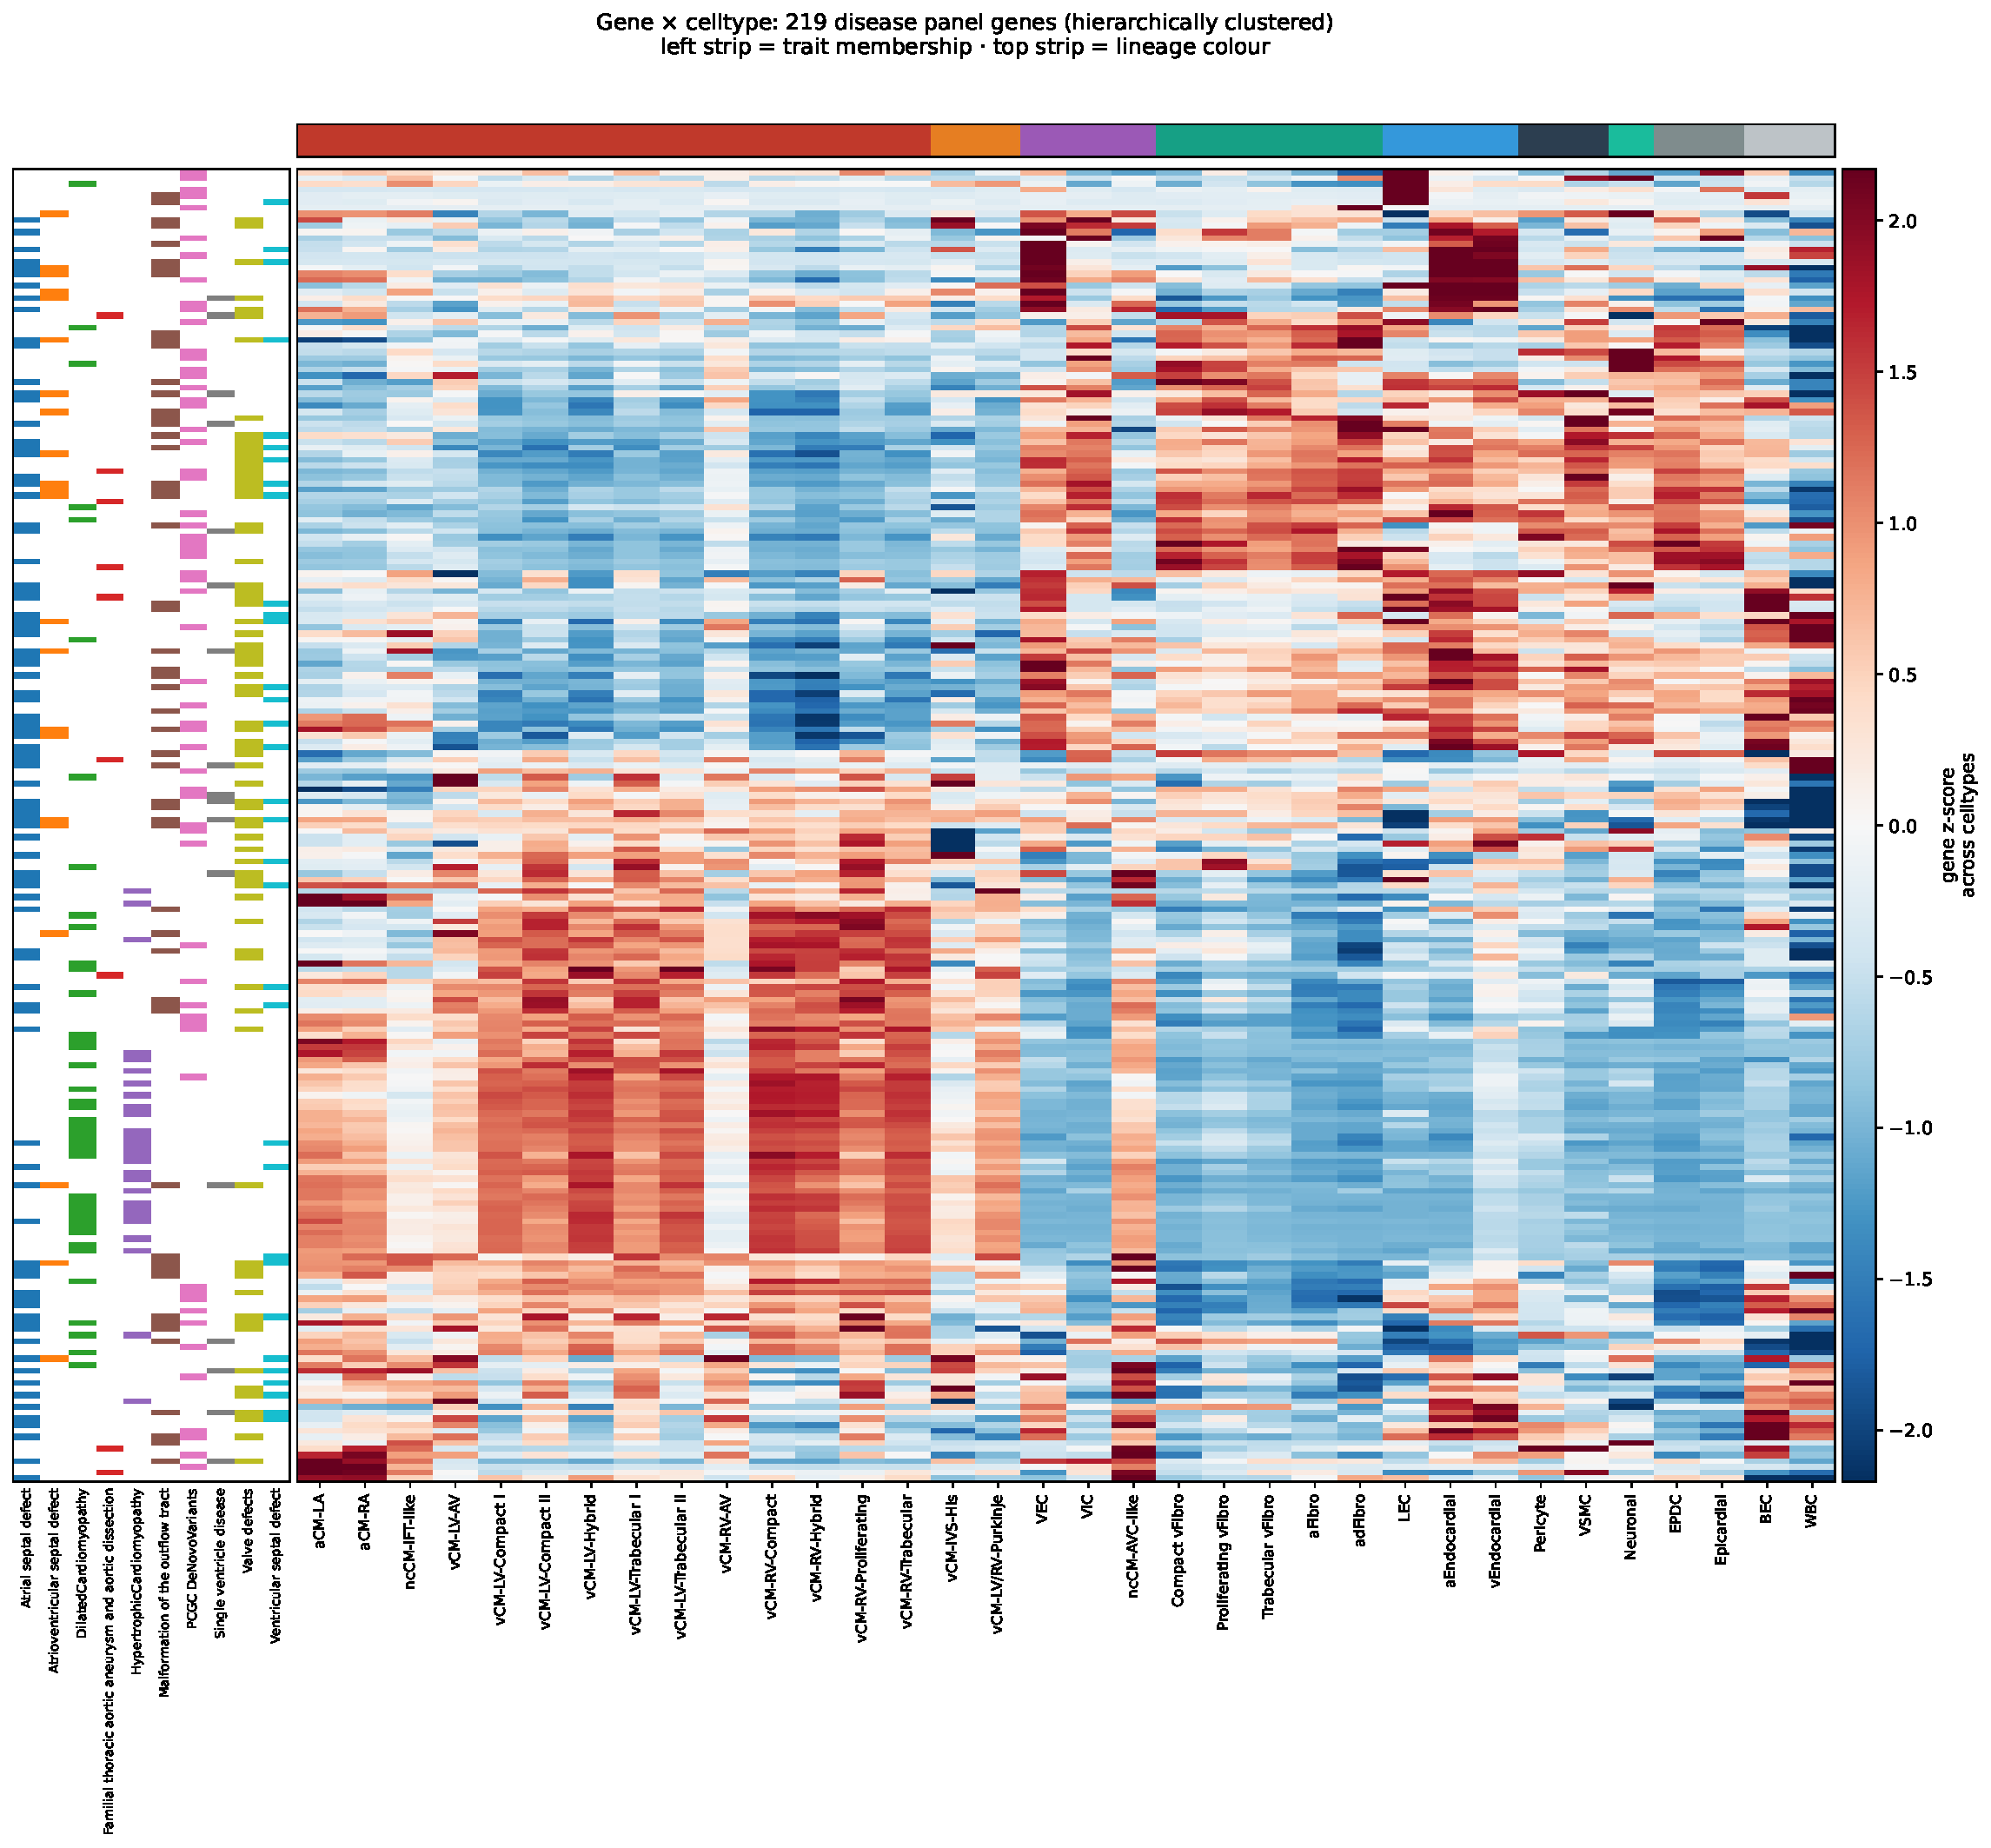
\includegraphics[width=0.95\linewidth]{figB_gene_by_celltype.pdf}
    \caption{\textbf{Gene-by-celltype heatmap, hierarchically clustered.}
    Rows: 219 disease genes (Ward linkage on $z$-scored rows). Three
    dominant gene modules emerge from the row dendrogram: M-CM
    (working-myocyte specific; HCM/DCM heavy), M-cushion (VEC/VIC/
    Endocardial; valve and septal CHD), and M-mesenchymal (Fibroblast/
    VSMC/LEC; TAA + PCGC).}
    \label{fig:B}
\end{figure}

\begin{table}[H]
    \centering\small
    \begin{tabularx}{\linewidth}{@{}l Y Y@{}}
        \toprule
        \textbf{Module} & \textbf{Where it lights up} & \textbf{Trait membership} \\
        \midrule
        M-CM           & all vCM subtypes red, valve/EC/fibro blue                & HCM, DCM, plus CM-expressed PCGC/CHD genes \\
        M-cushion      & VEC, VIC, ncCM-AVC-like, aEndocardial, vEndocardial red & Valve\_defects, AVSD, OFT, ASD, VSD \\
        M-mesenchymal  & LEC, aEndocardial, VSMC, Fibroblasts red                 & TAA, PCGC, scattered CHD \\
        \bottomrule
    \end{tabularx}
    \caption{Three unsupervised gene modules (Fig.~\ref{fig:B}) and
    their trait associations. Module recovery from clustering alone ---
    without using trait labels in the distance --- is a non-trivial
    consistency check on the panel curation.}
    \label{tab:modules}
\end{table}

\subsubsection{Gene specificity: developmental TFs vs.\ chromatin regulators}

\begin{figure}[H]
    \centering
    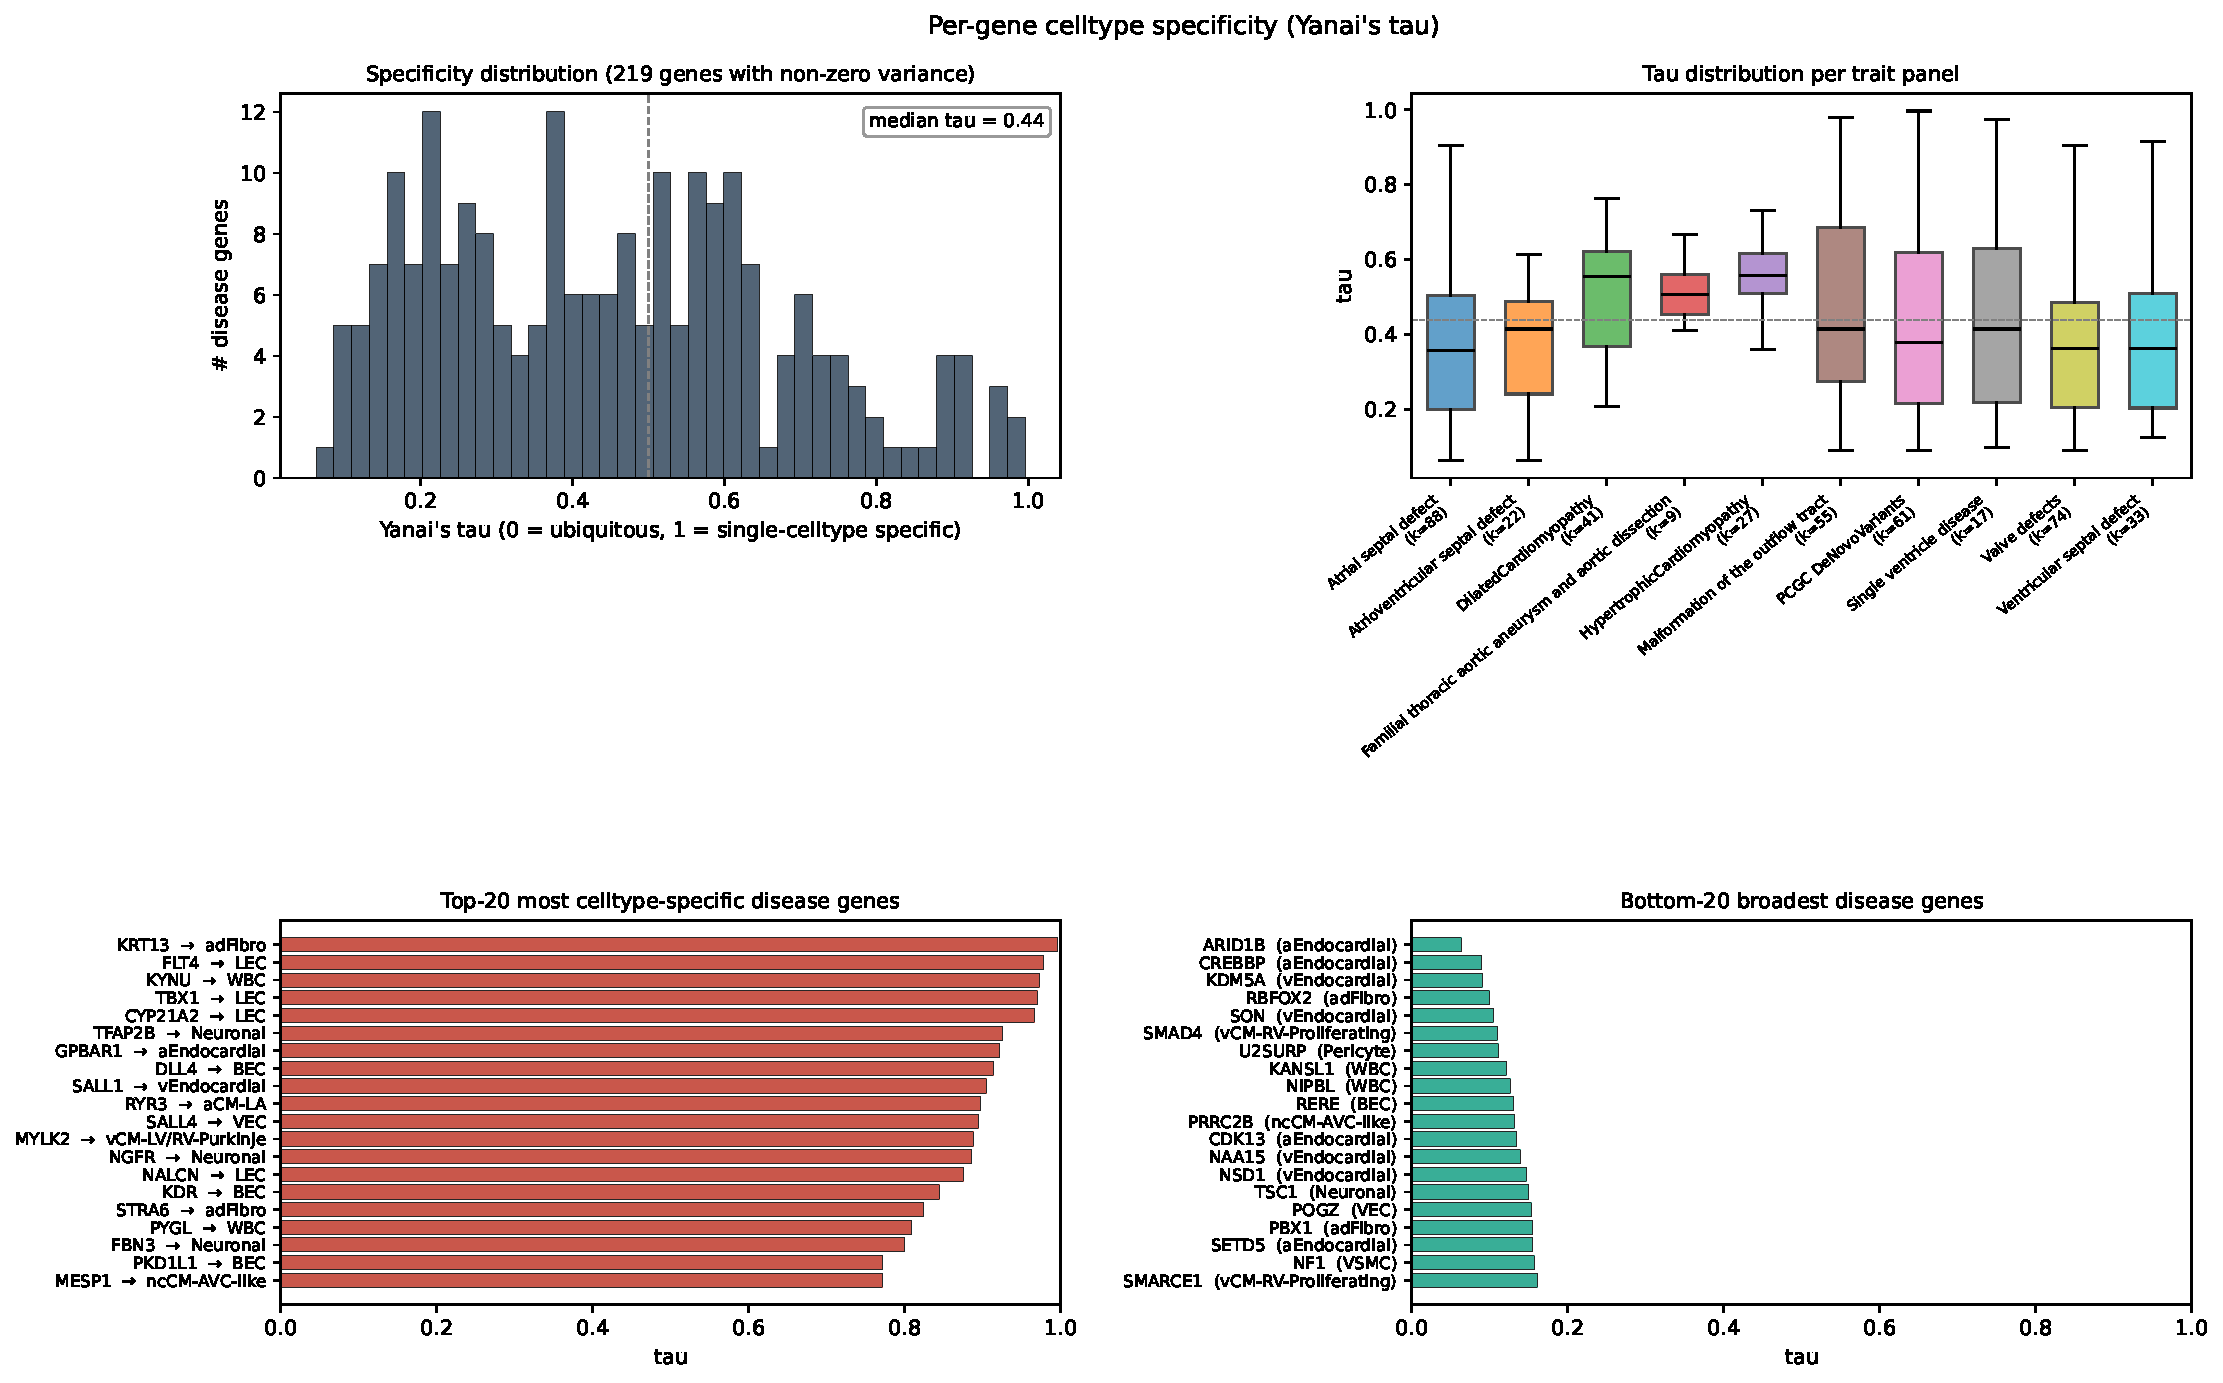
\includegraphics[width=0.95\linewidth]{figC_gene_specificity.pdf}
    \caption{\textbf{Per-gene cell-type specificity.} \emph{Top-left:}
    histogram of Yanai's $\tau$ across 219 informative disease genes
    (median $\tau = 0.44$). \emph{Top-right:} per-trait $\tau$
    distributions. \emph{Bottom:} top-20 most-specific and most-broad
    disease genes with their best cell type.}
    \label{fig:C}
\end{figure}

\begin{table}[H]
    \centering\small
    \begin{tabular}{@{}llrl@{}}
        \toprule
        \textbf{Gene} & \textbf{Best celltype} & \textbf{$\tau$} & \textbf{Biology} \\
        \midrule
        TBX1     & LEC                       & 0.970 & DiGeorge / 22q11 master regulator \\
        FLT4     & LEC                       & 0.978 & VEGFR3, lymphangiogenesis \\
        DLL4     & BEC                       & 0.914 & Notch ligand, arterial-EC marker \\
        KDR      & BEC                       & 0.844 & VEGFR2, pan-endothelial \\
        SALL1    & vEndocardial              & 0.905 & Townes--Brocks; endocardial cushion \\
        SALL4    & VEC                       & 0.894 & Okihiro / Duane-radial-ray; valve EC \\
        TFAP2B   & Neuronal                  & 0.925 & Char syndrome; neural-crest TF \\
        MYLK2    & vCM-LV/RV-Purkinje        & 0.888 & \textbf{HCM panel; \emph{Purkinje}-restricted} \\
        RYR3     & aCM-LA                    & 0.897 & Atrial-CM Ca$^{2+}$ release isoform \\
        CYP21A2  & LEC                       & 0.966 & Adrenal steroidogenesis \\
        \bottomrule
    \end{tabular}
    \caption{Selected high-$\tau$ disease genes. Cell-type assignments
    recapitulate canonical lineage markers --- a consistency check on
    imputed expression and cell-type curation.}
    \label{tab:high_tau}
\end{table}

\begin{tcolorbox}
\textbf{Mechanism tracks specificity.} High-$\tau$ disease genes are
tissue-program genes (TFs, signalling receptors, lineage markers);
low-$\tau$ disease genes are chromatin / splicing regulators (ARID1B,
CREBBP, KDM5A, KANSL1, NIPBL, NSD1, SETD5, SMARCE1, RBFOX2, NF1, PBX1,
TSC1, NAA15, POGZ). The same dichotomy that organises the molecular
basis of CHD genetics --- structural lineage genes vs.\ developmental
dosage regulators --- is visible in the $\tau$ histogram of a single
PCW12 atlas.
\end{tcolorbox}

\subsubsection{Trait similarity: convergence via independent genes}

\begin{figure}[H]
    \centering
    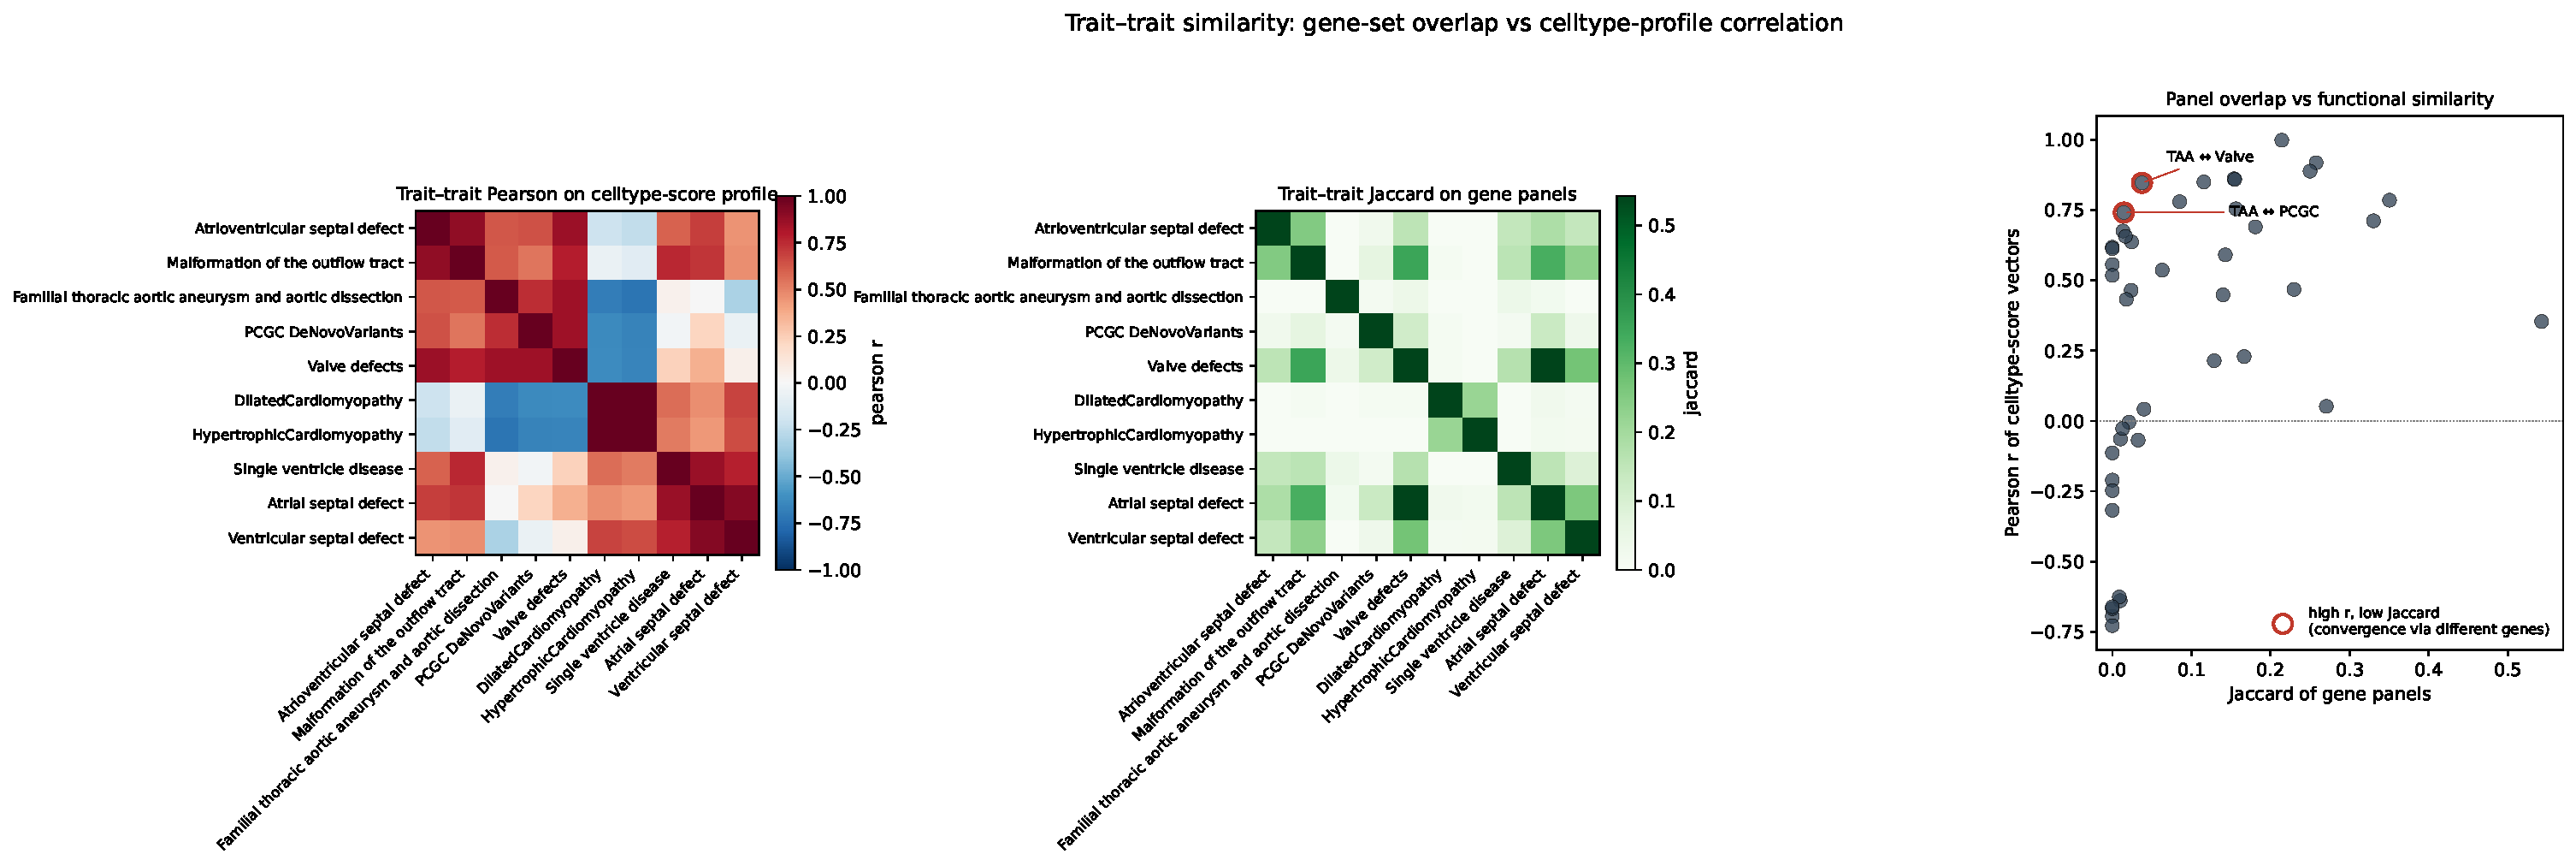
\includegraphics[width=0.97\linewidth]{figD_trait_similarity.pdf}
    \caption{\textbf{Trait--trait similarity.} \emph{Left:} Pearson
    correlation of celltype-score profiles. \emph{Middle:} Jaccard
    overlap of gene-membership sets. \emph{Right:} $r$ vs.\ $J$
    scatter, with annotated pairs in the high-$r$ / low-$J$ regime.
    The cushion-mesenchymal block correlates strongly even when
    gene-set overlap is near zero.}
    \label{fig:D}
\end{figure}

\begin{table}[H]
    \centering\small
    \begin{tabular}{@{}lrrrl@{}}
        \toprule
        \textbf{Pair} & \textbf{$r$} & \textbf{$J$} & \textbf{$|\mathcal{G}_1\cap\mathcal{G}_2|$} & \textbf{Reading} \\
        \midrule
        HCM $\leftrightarrow$ DCM             & 0.998 & 0.21 & 12 & Identical celltype profile, 21\% panel overlap \\
        ASD $\leftrightarrow$ VSD             & 0.92  & 0.26 & 25 & Overlapping septal panels \\
        \textbf{TAA $\leftrightarrow$ Valve\_defects} & \textbf{0.85} & \textbf{0.037} & \textbf{3} & \textbf{Functional convergence via different genes} \\
        TAA $\leftrightarrow$ PCGC            & 0.75  & $\sim$0.03 & $\sim$2 & Same convergence on mesenchymal program \\
        AVSD $\leftrightarrow$ Valve\_defects & 0.78  & 0.10 & 7 & Cushion overlap, partly shared \\
        \bottomrule
    \end{tabular}
    \caption{Selected trait pairs ranked by Pearson $r$. Full 45-pair
    table in \texttt{trait\_similarity.tsv}.}
    \label{tab:trait_pairs}
\end{table}

The TAA $\leftrightarrow$ Valve\_defects pair is the headline finding.
Two independently curated panels with \textbf{only 3 genes in common}
produce nearly indistinguishable celltype-score profiles ($r=0.85$).
At the panel level, TAA and Valve\_defects index the \emph{same
cushion-mesenchymal developmental program} through almost
non-overlapping gene sets. This reconciles the cell-level robustness
result in \S\ref{sec:res:stats}: TAA is a generic mesenchymal signature,
not valve-specific, but it shares the broader cushion-mesenchymal
program with the curated valve panel.

% =========================================================================
\section{Discussion}
\label{sec:discussion}

\paragraph{1. The disease panel decomposes into three developmental compartments.}
Working myocardium, AV/OFT cushion mesenchyme, and aortic / general
mesenchyme. The decomposition is recovered by hierarchical clustering
alone (Fig.~\ref{fig:B}, \S\ref{sec:res:landscape}), independent of trait
labels, and tracks the trait--trait similarity structure of
Fig.~\ref{fig:D}. This is biologically sensible: cardiomyopathies
originate in differentiated myocytes; septal and valvar CHD originate in
cushion-derived endothelial-to-mesenchymal transition; aortopathies in
neural-crest-derived smooth muscle and adventitial fibroblasts. The
peak-cell-type assignment (\S\ref{sec:res:peak}) lays out the same
decomposition in a different basis.

\paragraph{2. Cardiomyopathy panels collapse to a single celltype identity.}
HCM and DCM are indistinguishable as celltype-score profiles
($r=0.998$). They differ in genes (Jaccard $0.21$), but both panels
converge on the same working-myocyte celltype --- a result that surfaces
in three independent views: the heatmap (Fig.~\ref{fig:A}), the trait
similarity (Fig.~\ref{fig:D}), and as the joint depletion against valve
cells (Table~\ref{tab:stats}; AUC $0.18$ in both, $\log_2$FC $-1.4$ and
$-2.0$).

\paragraph{3. Convergent celltype targeting through non-overlapping gene sets.}
The TAA $\leftrightarrow$ Valve\_defects pair (3 shared genes,
$r = 0.85$) and the TAA $\leftrightarrow$ PCGC pair argue that disease
loci across phenotypes tag a shared developmental program (here,
EMT-derived cushion / aortic mesenchyme), rather than capturing
trait-specific biology by gene-set enrichment artefact. The valve-test
caveat (\S\ref{sec:res:stats}) and the trait-similarity result
(\S\ref{sec:res:landscape}) reinforce each other: at the cell level TAA
is non-valve-specific, at the celltype-profile level it is functionally
indistinguishable from Valve\_defects.

\paragraph{4. Mechanism tracks specificity.}
High-$\tau$ disease genes are tissue-program genes (TFs, signalling
receptors, lineage markers); low-$\tau$ disease genes are dosage-sensitive
chromatin / splicing regulators. The same dichotomy that organises CHD
genetics --- structural lineage genes vs.\ developmental dosage
regulators --- is visible in the $\tau$ histogram of a single PCW12
atlas (Fig.~\ref{fig:C}).

\paragraph{Practical follow-ups suggested by the data.}
\begin{enumerate}[leftmargin=*,itemsep=1pt]
    \item \emph{Stratify the HCM panel by cell type.} MYLK2 is
          Purkinje-restricted at PCW12; subset analyses that separate
          working-myocyte from conduction-system HCM members may resolve
          disease-mechanism heterogeneity.
    \item \emph{Replace the TAA panel with a derived
          mesenchymal-cushion meta-signature} for downstream enrichment;
          would absorb TAA, Valve\_defects, PCGC, and AVSD signal cleanly.
    \item \emph{Use BEC and WBC as biological negative-control celltypes}
          in any downstream gene-set test on this atlas.
    \item \emph{Try alternate symbols} for the 6 missing genes
          (TAFAZZIN $\to$ TAZ; ZIC3 likely a casing/symbol mismatch).
\end{enumerate}

% =========================================================================
\section{Limitations}
\label{sec:limitations}

\begin{itemize}[leftmargin=*,itemsep=1pt]
    \item \textbf{Single donor, two batches.} All findings describe one
          PCW12 specimen; donor-level pseudoreplication is not possible.
          Generalisation to other donors and developmental times is out
          of scope.
    \item \textbf{MOSCOT mapping confidence is moderate}
          (mean $0.487$). Imputation recovers cell-type-level patterns
          well but smooths out single-cell variability; per-cell calls
          on imputed values should not be over-interpreted.
    \item \textbf{Imputed expression inherits scVI-style smoothing.}
          Cell-cell correlations would inflate raw Mann--Whitney $p$;
          we therefore report permutation $q_{\text{perm}}$ as the
          headline statistic --- it reuses the same imputed matrix for
          the null and is robust to this.
    \item \textbf{Small, CHD-biased panel.} The 221-gene universe is
          small. $\tau$ here is an \emph{intra-panel} specificity, not
          genome-wide; a $\tau=0.5$ here is not directly comparable to
          one computed over $\sim$20{,}000 genes. The permutation null
          for the valve test is drawn from the same biased pool, which
          is the correct null for ``given this CHD-relevant panel''.
    \item \textbf{6 missing genes} are excluded from spatial analyses.
\end{itemize}

% =========================================================================
\section*{Data and code availability}
\addcontentsline{toc}{section}{Data and code availability}

All paths are relative to the project root
\texttt{pantheonos-reproducibility/human-heart}.

\paragraph{Pipeline.} Twelve numbered scripts under
\texttt{PCW12\_analysis/scripts/}:

\begin{table}[H]
    \centering\small
    \begin{tabularx}{\linewidth}{@{}l Y@{}}
        \toprule
        \textbf{Script} & \textbf{Phase} \\
        \midrule
        \texttt{01\_partition\_genes.py}                          & gene partitioning (20 / 221 / 6) \\
        \texttt{02\_direct\_visualization.py}                     & direct 3D PNG + GIF \\
        \texttt{03\_moscot\_imputation.py}                        & MOSCOT OT mapping ($\sim$12 min, CPU) \\
        \texttt{04\_imputed\_visualization.py}                    & imputed 3D PNG + GIF + heatmaps \\
        \texttt{05\_data\_overview.py}                            & QC and cross-modal overview \\
        \texttt{05\_category\_aggregation.py}                     & per-category aggregated trait map \\
        \texttt{05b\_trait\_aggregation.py}                       & per-trait aggregated 3D map \\
        \texttt{06\_mapping\_heatmap.py}                          & SC $\to$ MERFISH transport heatmap \\
        \texttt{07\_trait\_celltype\_heatmap.py}                  & trait $\times$ celltype clustermap \\
        \texttt{08\_disease\_genes\_celltype\_heatmap.py}         & gene $\times$ celltype clustermap \\
        \texttt{09\_disease\_genes\_peak\_celltype\_barplot.py}   & peak-celltype assignment \\
        \texttt{10\_section16\_valve\_spatial.py}                 & section-16 valve spatial \\
        \texttt{11\_valve\_enrichment\_stats.py}                  & MWU + permutation null + BH-FDR \\
        \texttt{12\_disease\_gene\_landscape.py}                  & landscape ($\tau$, Pearson, Jaccard) \\
        \bottomrule
    \end{tabularx}
\end{table}

\paragraph{Inputs.}
\begin{itemize}[leftmargin=*,itemsep=1pt]
    \item \texttt{data/all\_healthy\_RoundedPCW11-13.h5ad}
    \item \texttt{data/full\_heart\_final\_aug2025\_update\_downsampled\_100k.h5ad}
    \item \texttt{data/heart\_disease\_genes.tsv}
\end{itemize}

\paragraph{Key derived files.}
\begin{itemize}[leftmargin=*,itemsep=1pt]
    \item \texttt{PCW12\_analysis/data/disease\_genes\_partition.tsv} (247 rows)
    \item \texttt{PCW12\_analysis/data/adata\_imputed\_disease\_genes.h5ad} (100k $\times$ 221, 274 MB)
    \item Figure subdirectories under \texttt{PCW12\_analysis/figures/}: \texttt{overview/}, \texttt{direct/}, \texttt{imputed/}, \texttt{heatmaps/}, \texttt{category\_aggregated/}, \texttt{trait\_aggregated/}, \texttt{barplots/}, \texttt{spatial\_section/}, \texttt{valve\_enrichment\_stats/}, \texttt{disease\_gene\_landscape/}.
    \item Tables: \texttt{trait\_by\_celltype\_means.tsv} ($10\times34$), \texttt{gene\_specificity\_tau.tsv} (221), \texttt{trait\_similarity.tsv} (45 pairs), \texttt{disease\_gene\_peak\_celltype\_counts.tsv}, \texttt{valve\_enrichment\_stats.tsv} ($10\times16$), \texttt{valve\_enrichment\_by\_subtype.tsv}, \texttt{valve\_vs\_fibroblast.tsv}, \texttt{section\_valve\_enrichment.tsv}.
\end{itemize}

\paragraph{Reproduce.}
\begin{verbatim}
cd $ROOT  # pantheonos-reproducibility/human-heart
for s in PCW12_analysis/scripts/[0-9]*.py; do
    python $s
done
\end{verbatim}
Total runtime $\sim$15 min (MOSCOT mapping is the rate-limiting step;
all other phases finish in $<$1 min each).

\end{document}
